\documentclass{beamer}
\usepackage[utf8]{inputenc}
\usepackage{graphicx}
\usepackage{multimedia}
\usepackage{url}

\usetheme{default}
\usecolortheme{crane}
\usefonttheme{default}
\useoutertheme{sidebar}
\useinnertheme[shadow=true]{rounded}

\title{Jeu du Pérudo}
\author{H4104 - Dragibus}
\institute{INSA de Lyon}
% \logo{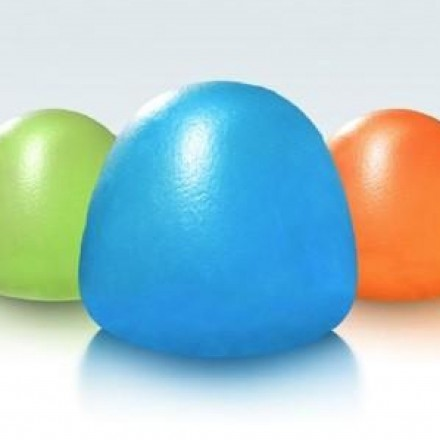
\includegraphics[height=8mm]{logo.jpeg}}

% \AtBeginSection[]
% {
%     \begin{frame}
%     \frametitle{Sommaire}
%     \tableofcontents[currentsection, hideothersubsections]
%     \end{frame}
% }

\begin{document}

\begin{frame}
    \titlepage
\end{frame}

\begin{frame}
    \frametitle{Sommaire}
    \tableofcontents[hideallsubsections]
\end{frame}

\section{Mécanisme du jeu}

\begin{frame}
    \frametitle{Principe}
    \begin{itemize}
        \item jeu de dés
        \item multijoueur, entre 2 et 6 (ou plus) joueurs
        \item deviner le nombre de dés d'une valeur, connaissant seulement ses propres dé
        \item dernier joueur ayant des dés gagne la partie
    \end{itemize}
\end{frame}

\begin{frame}
\frametitle{Règles}
    $\to$ parier sur le nombre de dés en jeu \\
    \emph{(pour une certaine valeur de dé)}

    \begin{itemize}
        \item enchêre
        \item dudo
        \item calza
    \end{itemize}
\end{frame}

\begin{frame}
    \frametitle{Exemple}

    % TODO formatter cette slide

    \begin{center}
        \begin{large}
            Joueur précédent : \textit{"Je pense qu'il y a douze 5"} \\
            \uncover<2>{Moi :\textit{"Je pense qu'il y a treize 5"}}
        \end{large}
    \end{center}

    $\to$ la mise ne peut qu'\textbf{augmenter} au cours de la partie
\end{frame}

\section{Concept d'IA}

\begin{frame}
    \frametitle{Constat}

    \begin{large}
        À son tour, le joueur doit \textbf{évaluer} les différents coups possibles.
    \end{large}

\end{frame}

\begin{frame}
    \frametitle{Constat}

    \huge Les

\end{frame}

\begin{frame}
    \frametitle{Combinaison}
\end{frame}

\section{Présentation des IA}

\section{Résultats et observations}

\end{document}
